\begin{center}
Лабораторная работа №1.
\\
Тема: Работа с системами контроля версий.
\\
Цель: Изучить порядок клонирования репозитория на гитхабе и на компьютере.
 
\end{center}
Задание:
\begin{enumerate}
\item Зарегистрироваться на https://github.com/

\item Склонировать репозиторий шаблонов tex https://github.com/egorpugin/tex
 
\item Подготовить шаблон отчёта для лабораторных работ в LaTeX.

\item Загрузить шаблон в репозиторий tex.

\item Создать новый репозиторий для лабораторных работ на гитхабе.

\item Оформить отчёт и загрузить его в репозиторий для ЛР.
\end{enumerate}
Ход выполнения:
\\
Порядок клонирования репозитория на компьютере.

\begin{figure}[h]
\centering
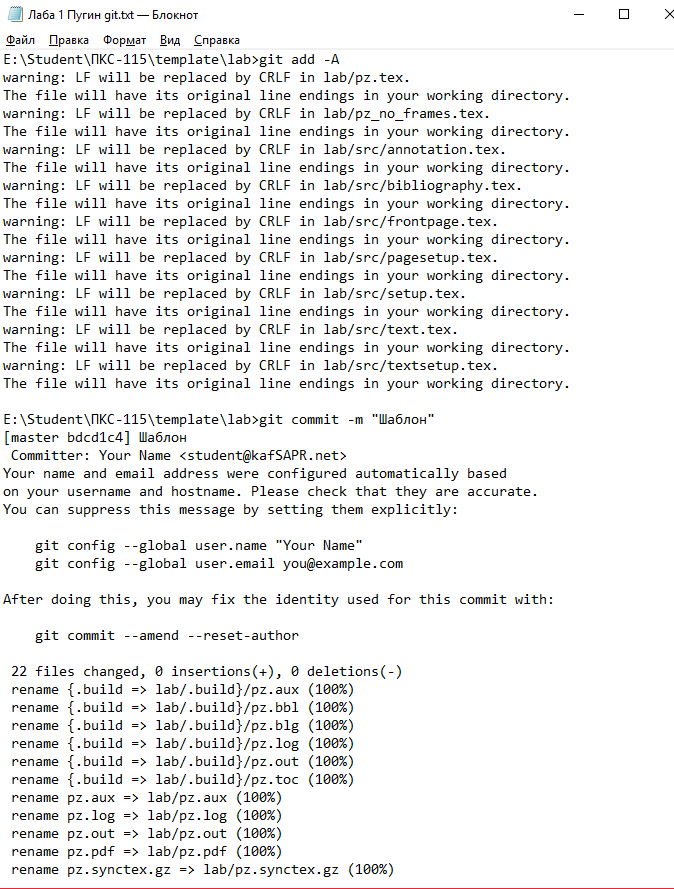
\includegraphics[scale=1]{l1}

\label{fig:l1}
\end{figure}

\begin{figure}[h]
\centering
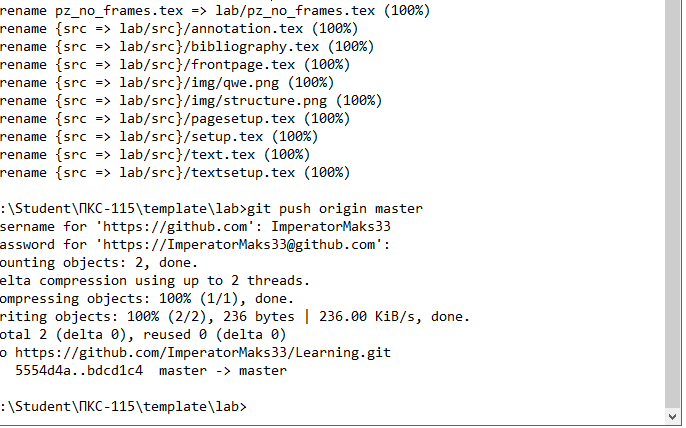
\includegraphics[scale=1]{l2}

\label{fig:l2}
\end{figure}

\begin{figure}[h]
\centering
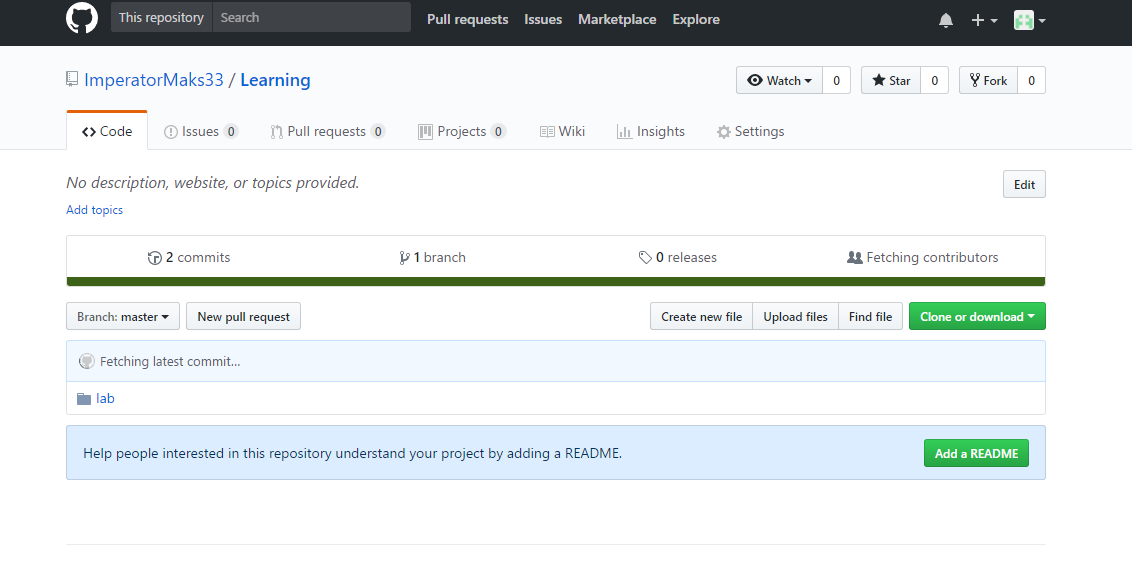
\includegraphics[scale=0.6]{l3}

\label{fig:l3}
Вывод: Изучил порядок клонирования репозитория на гитхабе и на компьютере.
\end{figure}



